\makeatletter\let\ifGm@compatii\relax\makeatother
\documentclass[a4,11pt]{beamer}
\usepackage[utf8]{inputenc} % this is needed for umlauts
\usepackage[ngerman]{babel} % this is needed for umlauts
\usepackage[T1]{fontenc}
\usepackage{url}
\usepackage{hyperref}


\usepackage{framed,color,verbatim}
\definecolor{shadecolor}{rgb}{.9, .9, .9}

\newenvironment{code}%
   {\small\snugshade\verbatim}%
   {\endverbatim\endsnugshade}




%\input{lmu_setup_new}
\usepackage{tikz}
\usepackage{booktabs}
\usepackage{graphicx}
%\usepackage[round]{natbib}
\usepackage{multirow}
\usepackage{tikz}
    \usetikzlibrary{trees}
    \usetikzlibrary{decorations.pathmorphing}
    \usetikzlibrary{shapes,arrows,matrix}
		\usetikzlibrary{petri}
		\usetikzlibrary{automata,positioning}
		\usetikzlibrary{decorations.pathreplacing}
%		\usetikzlibrary{quotes,angles}
		\usetikzlibrary{calc,patterns,angles,quotes}
		
\graphicspath{{graphics/}}
%\input{LaTeX/defs}
%\input{LaTeX/symbole}

\usepackage{appendixnumberbeamer}
\usepackage{bm}

\definecolor{sixtyeight}{RGB}{4,90,141}
 \definecolor{look}{RGB}{4,90,141}
 
\newcommand\independent{\protect\mathpalette{\protect\independenT}{\perp}}
\def\independenT#1#2{\mathrel{\rlap{$#1#2$}\mkern2mu{#1#2}}}

\definecolor{seventyeight}{RGB}{43,140,190}
\definecolor{eightyeight}{RGB}{116,169,207}
\definecolor{ninetyyeight}{RGB}{189,201,225}
\definecolor{blueberry_light}{RGB}{188,189,220}
%208,209,230 blueberry light
\definecolor{blueberry_very_light}{RGB}{218,218,235}
\definecolor{blueberry_very_very_light}{RGB}{239,237,245}
\definecolor{look}{RGB}{2,129,138}
\definecolor{blueberry}{RGB}{0,0,153}
\definecolor{counterfactual}{RGB}{253,140,37}
\definecolor{cobalt}{RGB}{0,71,171}
\mode<presentation>
 {
 \usetheme{CambridgeUS}
 \setbeamercolor{titlelike}{parent=structure, fg = blueberry, bg = blueberry_very_light}
 \setbeamercolor*{palette secondary}{use=structure,fg=white,bg=blueberry_light}
 \setbeamercolor*{palette tertiary}{use=structure,fg=white,bg=blueberry}
\setbeamercolor{palette primary}{fg=blueberry,bg=blueberry_very_light} % changed this
 \setbeamercolor{frametitle}{fg=blueberry,bg=blueberry_very_very_light}
\setbeamercolor{section in head/foot}{bg=blueberry}
\setbeamercolor{author in head/foot}{bg=blueberry}
\setbeamercolor{date in head/foot}{fg=blueberry}
 }


   
 %\renewcommand{\baselinestretch}{1.5}\normalsize
\newcommand\X{\bf X}
\newcommand\x{\bf x}
\newcommand{\R}{\mathbb{R}}
\newcommand{\E}{\mathbb{E}}
%\newcommand{\Pr}{\mathds{P}}
\def\Y{\boldsymbol Y}


\usetikzlibrary{shapes,arrows}
\tikzstyle{every picture}+=[remember picture]
\newlength{\wideitemsep}
\setlength{\wideitemsep}{\itemsep}
\addtolength{\wideitemsep}{15pt}
\let\olditem\item
\renewcommand{\item}{\setlength{\itemsep}{\wideitemsep}\olditem}

\usepackage{graphicx,calc}
\newlength\myheight
\newlength\mydepth
\settototalheight\myheight{Xygp}
\settodepth\mydepth{Xygp}
\setlength\fboxsep{0pt}



\newcommand{\N}{\mathbb{N}}
\newcommand{\pr}{\ensuremath{\operatorname{P}}}
\newcommand{\diff}{\mathrm{d}}
\newcommand{\supp}{\operatorname{supp}}
\newcommand{\var}{\operatorname{Var}}
\newcommand{\cov}{\operatorname{Cov}}
\newcommand{\corr}{\operatorname{corr}}
\usefonttheme{professionalfonts}
\usepackage{biblatex}

\addbibresource{refs.bib}


\definecolor{links}{RGB}{188,189,220}
\hypersetup{colorlinks,linkcolor=,urlcolor=links}
\begin{document}

	\title{Multivariate Verfahren}
	\subtitle{1. Some probability theory}
	
	
	\author[Hannah Schulz-Kümpel]{Hannah Schulz-Kümpel\bigskip\\
 Department of Statistics, LMU Munich}
	\date{}
	
	
	\institute[]{Summer semester 2024}
	\frame[plain]{
		\maketitle}


\begin{frame}{}
    \begin{center}
        \textcolor{blueberry}{\bfseries \emph{We will start at the very beginning: \\
The realm of probability theory!}}
    \end{center}
    \tableofcontents
\end{frame}
\begin{frame}{}\begin{minipage}{.35\linewidth}
     Quick set theory reminder: 
\end{minipage}%
\begin{minipage}{.65\linewidth}
    \vspace{-1.2cm}
  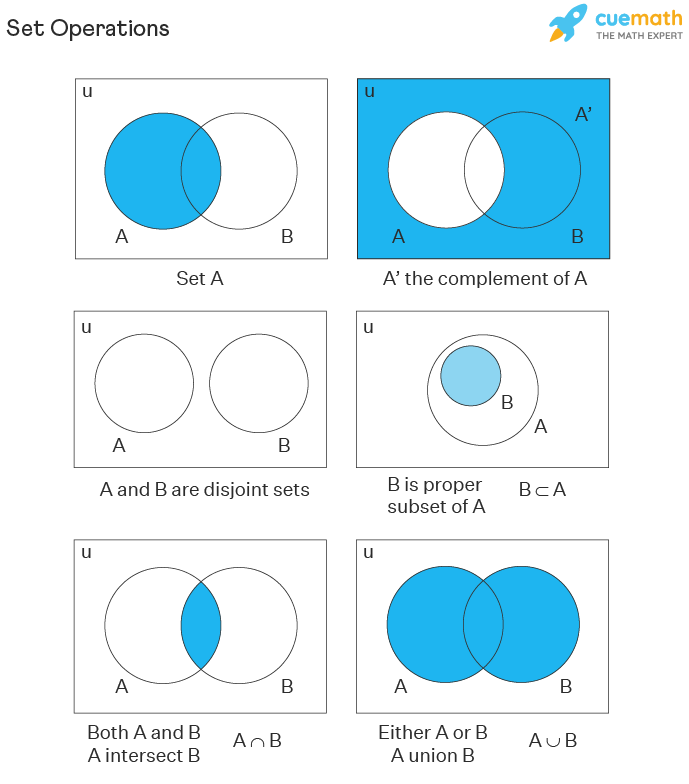
\includegraphics[height=\paperheight]{graphics/SetOperationsold.png}
\end{minipage}
\end{frame}

\section{Let's get philosophical}
\begin{frame}{}
    \begin{center}
        \textcolor{blueberry}{\textbf{\Large{QUESTION:}}}\bigskip\\

        \emph{\Large What is your understanding of the term "probability"?}
    \end{center}
\end{frame}
\begin{frame}{}
\begin{center}
        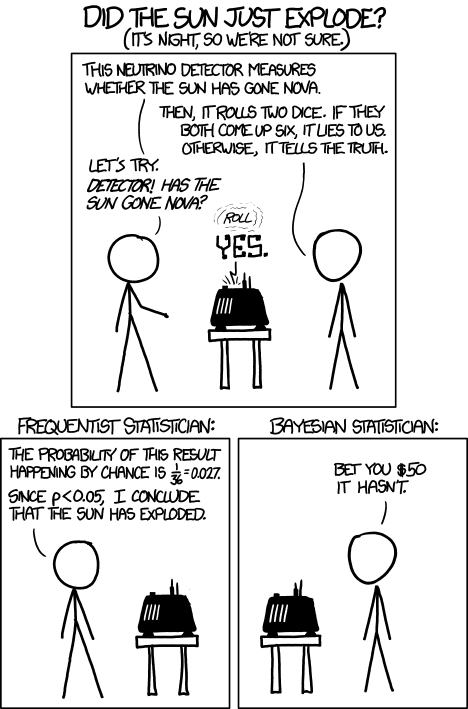
\includegraphics[height=.9\paperheight]{graphics/frequentists_vs_bayesians.png}
\end{center}
\end{frame}
\begin{frame}{Mathematics is here to help!}
    \begin{itemize}
        \item So is there no ''true'' definition of probability?!
        \item Actually, there are two equivalent ways of formalizing the concept of probability:\bigskip\\\begin{itemize}
            \item \textcolor{blueberry}{Cox's theorem}\vspace{-.1cm}\\
            \item \textcolor{blueberry}{The axioms of Kolmogorov (probability axioms)} \\
            $\rightarrow$ \emph{what we will focus on, since much more popular.}
        \end{itemize}
        \end{itemize}
        \end{frame}
        
\begin{frame}[allowframebreaks]{Kolmogorov axioms - heuristic version}
    \begin{minipage}{.6\linewidth}
        \begin{itemize}
            \item The axiomatic foundations of modern probability theory were laid \textcolor{blueberry}{only as recently as 1933}!
            \item Specifically, they were published in the book \emph{Foundations of the Theory of Probability} by Andrey Kolmogorov.
        \end{itemize}
    \end{minipage}%
    \begin{minipage}{.4\linewidth}
        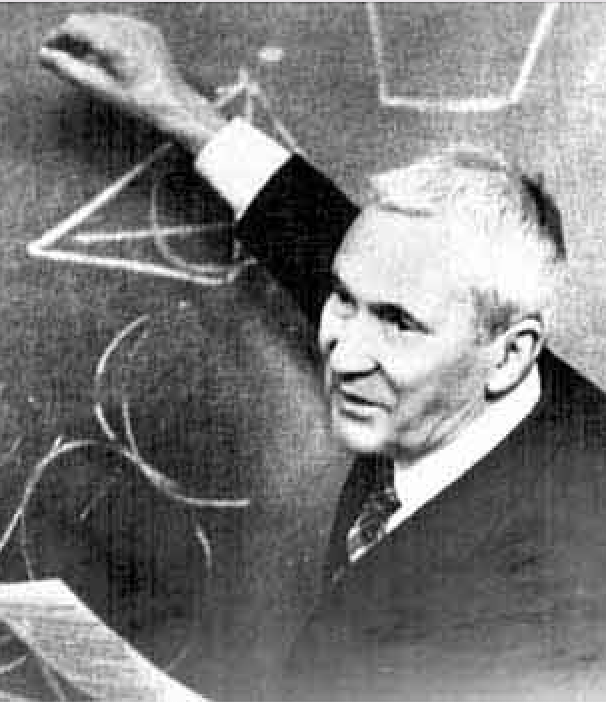
\includegraphics[width=\linewidth]{graphics/Kolmogorov.png}
    \end{minipage}\,\\\pagebreak
    \textbf{Heuristically}, for an event space $\mathcal{S}$, i.e. the set of all possible events, the axioms state the following:\bigskip\\
    
    \hspace*{1cm}\begin{minipage}{.9\linewidth}
     \begin{itemize}
        \item[Axiom 1:] For any event $E$, the probability of $E$ is greater or equal to zero.
        \item[Axiom 2:] The probability of the union of all events equals $1$.
        \item[Axiom 3:] For a countable sequence of mutually exclusive events $E_1,E_2,E_3,...$ the probability of any of these events occurring is equal to the sum of each of the events occurring.
    \end{itemize}   
    \end{minipage}
    
\end{frame}


\section{Probability spaces and operations}
  {
     \begin{frame}
     \frametitle{Contents}
     \tableofcontents[currentsection]
     \end{frame}
  }
\begin{frame}[allowframebreaks]{Formalizing probability}
        \begin{itemize}
        \item Of course, to derive the probability calculus and more complex results (like the CLT) which most of applied statistics is built on, we need a formal version of these axioms.
        \item Luckily, set- and measure- theory have us covered!
        \item We only need two definitions to get started:\pagebreak
        \begin{definition}[$\sigma$-Algebra]
        Given a set $S$, a collection $\mathcal{A}$ of subsets of $S$ is called \emph{$\sigma$-algebra over $S$}, if it satisfies the following properties:\begin{enumerate}
            \item $S\in\mathcal{A}$\vspace{-.5cm}\\
            \item $A\in\mathcal{A}\quad\Rightarrow\quad A^c\in\mathcal{A}\quad$ ($\mathcal{A}$ is closed under complementation)\vspace{-.5cm}\\
            \item For sets $A_1,A_2,A_3,...\in\mathcal{A}\Rightarrow\underset{i\in\N}{\bigcup}A_i\in\mathcal{A}$ ($\mathcal{A}$  is closed under countable unions)
        \end{enumerate}
        \end{definition}
        \item For countable sets $S$, the largest possible $\sigma$-algebra is the \textbf{power set}, i.e. the set containing all subsets of $S$, including the empty set and $S$ itself. The power set of $S$ is often denoted by $\mathcal{P}(S)$ or $2^S$.
    \end{itemize}
    \pagebreak
    \begin{minipage}{.2\linewidth}
        An example:
    \end{minipage}%
    \begin{minipage}{.6\linewidth}
    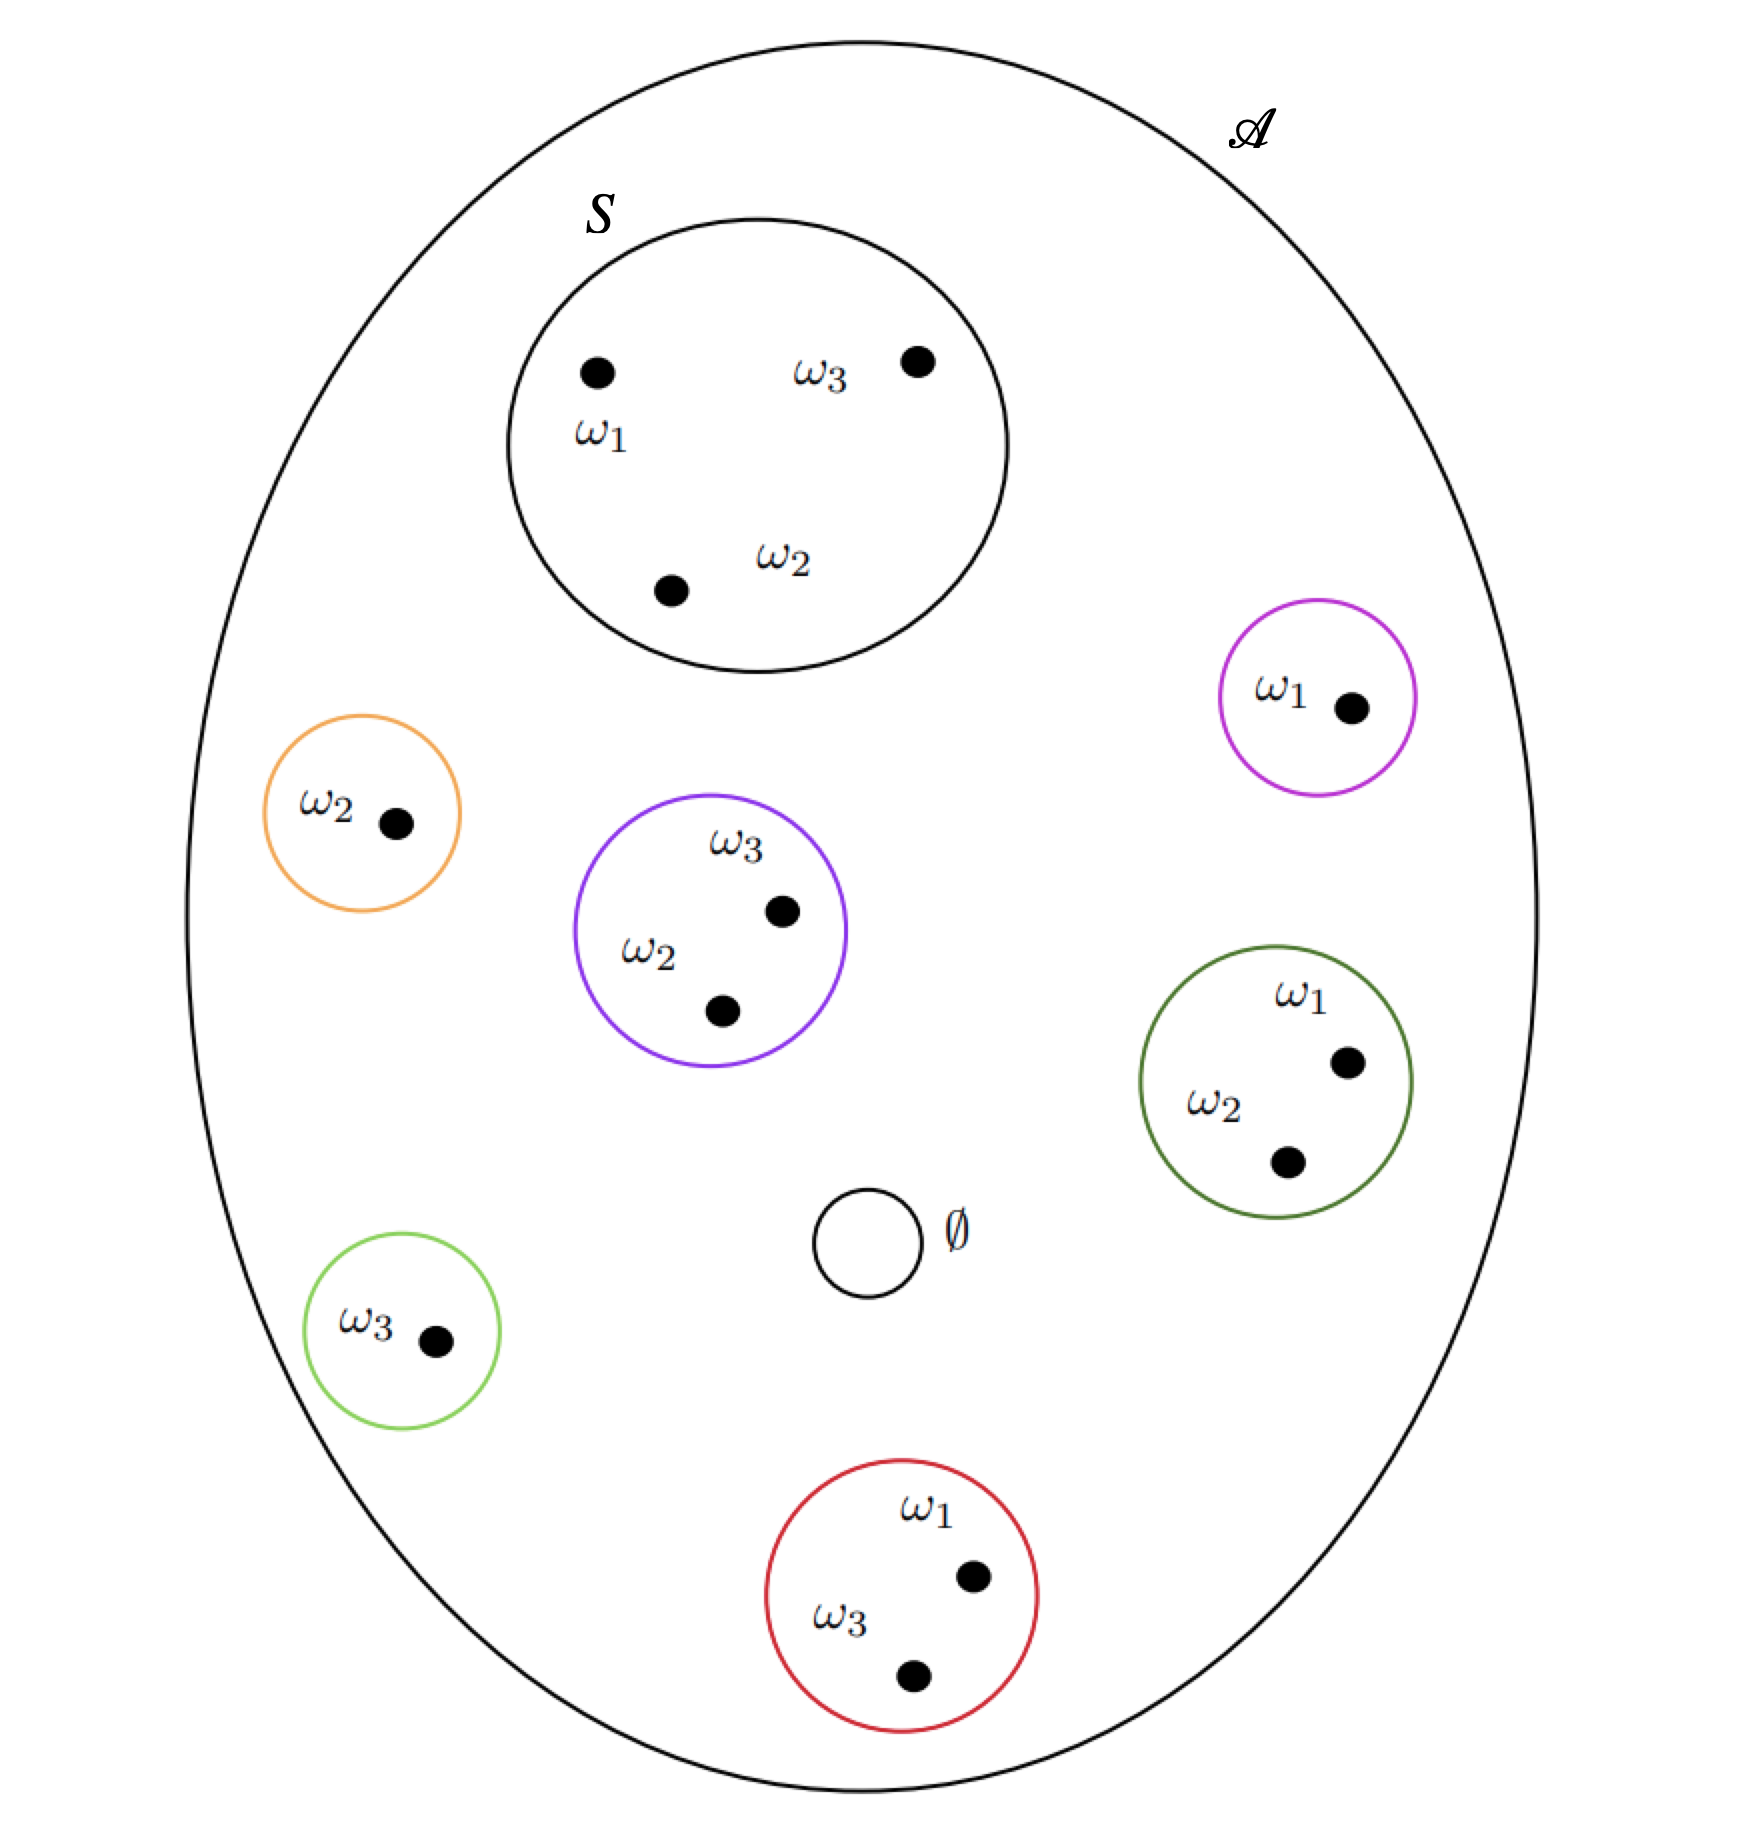
\includegraphics[width=\linewidth]{graphics/SigmaAlgebra.png}
    \end{minipage}%
    \begin{minipage}{.2\linewidth}
        $\quad \hat{=}\mathcal{P}(S)$
    \end{minipage}

    \begin{definition}[Measure]
        Consider a $\sigma$-algebra $\mathcal{A}$ over a set $S$. A function $\mu:\mathcal{A}\longrightarrow [0,\infty]$ that meets the following requirements
        \begin{enumerate}
            \item $\mu(\emptyset)=0$\vspace{-.5cm}\\
            \item $\forall A\in\mathcal{A}: \quad \mu(A)\geq 0$\vspace{-.5cm}\\
            \item For pairwise disjoint sets $A_1,A_2,A_3,...\in\mathcal{A}\quad\Rightarrow\quad\mu\big(\underset{i\in\N}{\bigcup}A_i\big)=\underset{i\in\N}{\sum}\mu(A_i)$.
        \end{enumerate} is called \emph{measure}.
        
    \end{definition}\,\\
\begin{itemize}
    \item\textcolor{blueberry}{\textbf{Example:} Cardinality.} \emph{We can easily check that the function that maps any set to the number of its elements fulfills the above definition of measure on $\sigma$-algebra $\mathcal{P}(S)$ for any finite set $S$.}\pagebreak
    \item So measures are mathematical objects that quantify some definition of set-size:
   \end{itemize} 
    \begin{center}\vspace*{-.3cm}
        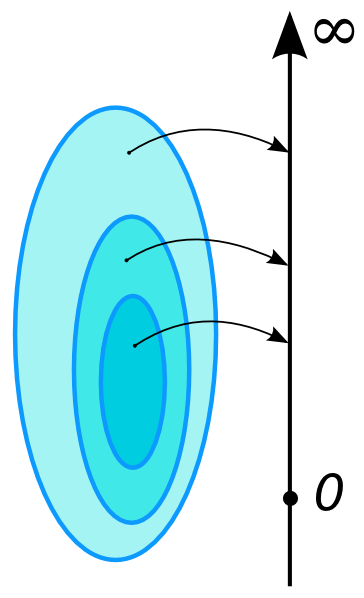
\includegraphics[width=.3\linewidth]{graphics/Measure_illustration.png}
      \resizebox{\linewidth}{!}{By Oleg Alexandrov - Own work based on: Measure illustration.png, Public Domain, \url{https://commons.wikimedia.org/w/index.php?curid=32489121}}   
    \end{center}
   
    
\pagebreak
\begin{itemize}    
        \item Having defined the concepts of \emph{$\sigma$-algebra} and \emph{measure}, we can formalize the Kolmogorov axioms by\smallskip\\\begin{itemize}
            \item representing events as sets and\vspace{-.5cm}\\
            \item defining probability as a measure.
        \end{itemize}
    
    \begin{definition}[Probability measure]
        Consider a $\sigma$-algebra $\mathcal{F}$ over a set $\Omega$. A measure $\pr:\mathcal{F}\longrightarrow [0,\infty]$ with $\pr(\Omega)=1$ is called a \textbf{probability measure} on $\mathcal{F}$.
    \end{definition}
    \item Note that by the definition of measure, the following has to hold for any probability measure: $\forall A\in\mathcal{F}:\,\pr(A)\in[0,1]$. This is why probability measures are often directly defined via $\pr:\mathcal{F}\longrightarrow [0,1]$.
    \end{itemize}
\end{frame}
\begin{frame}{Visualizing probability measures}
   \begin{center}
       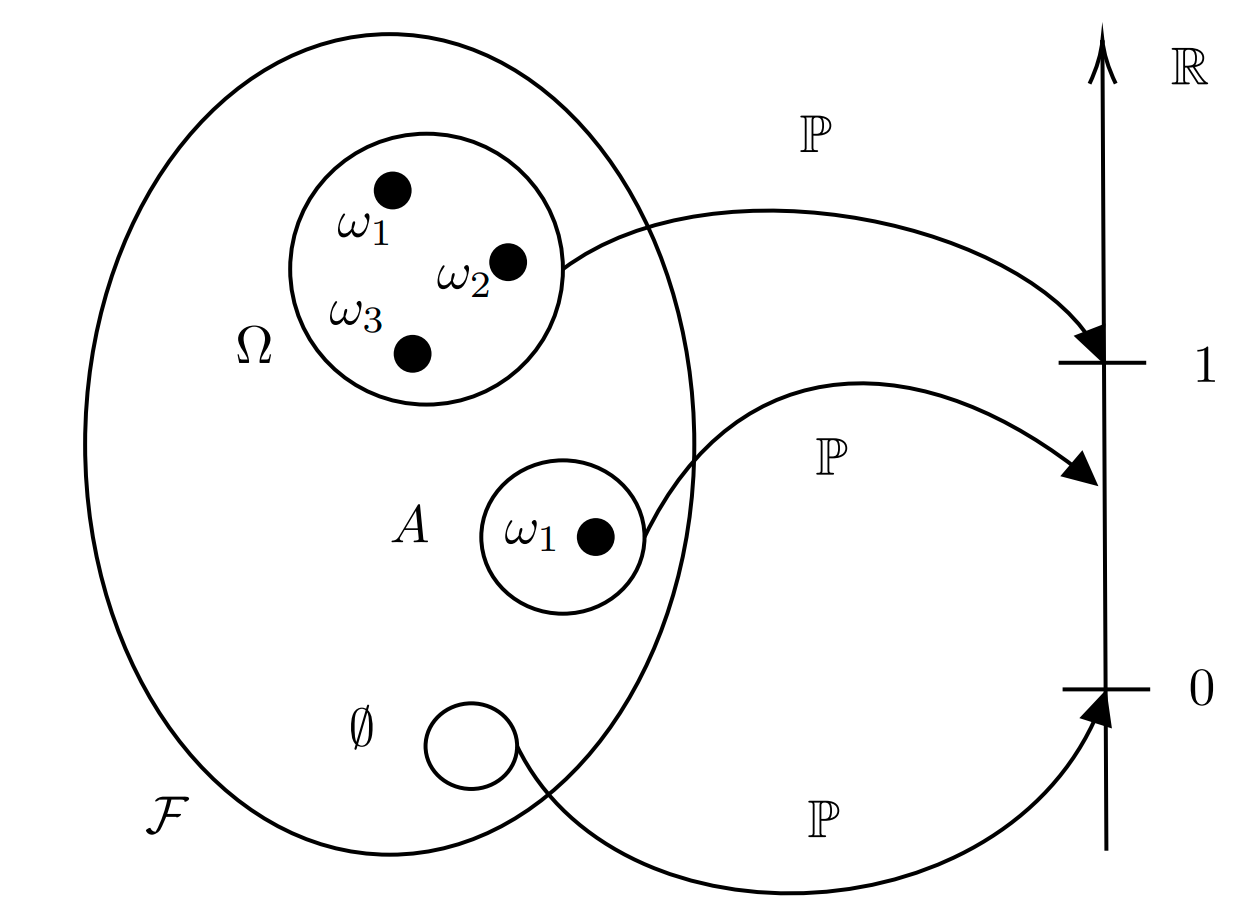
\includegraphics[width=.8\linewidth]{graphics/ProbabilityMeasure.png}\\
       {\tiny \textbf{Source:} \url{https://maurocamaraescudero.netlify.app/post/visualizing-measure-theory-for-markov-chains/}}
   \end{center} 
\end{frame}

\begin{frame}{Probability spaces}
\begin{definition}[Probability space]
    A probability space $\big(\Omega,\mathcal{F},\pr\big)$ consists of a nonempty set $\Omega$, a $\sigma$-algebra $\mathcal{F}$ over $\Omega$ and a probability measure $\pr$ on $\mathcal{F}$.
\end{definition}\,\\ Now, by the definition of $\sigma$-algebra and probability measure the Kolmogorov axioms automatically hold and can be formally expressed as follows:\bigskip\\
    \hspace*{.9cm}\begin{minipage}{.9\linewidth}
     \begin{itemize}
        \item[Axiom 1:] $\pr(A)\geq 0\quad \forall A\in\mathcal{F}$.
        \item[Axiom 2:] $\pr(\Omega)=1$.
        \item[Axiom 3:] For pairwise disjoint sets $A_1,A_2,A_3,...\in\mathcal{A}$ $\pr\big(\underset{i\in\N}{\bigcup}A_i\big)=\underset{i\in\N}{\sum}\pr(A_i)$.
    \end{itemize}   
    \end{minipage}

\end{frame}
{\usebackgroundtemplate{%
    \tikz[overlay,remember picture] 
  \node[opacity=0.5, at=(current page.south),anchor=south,inner sep=0pt] {
    
\includegraphics[height=.6\paperheight]{graphics/Gummy Bears.png}};}
\begin{frame}{Example: Gummy bears}
\vspace*{-3cm}
    \begin{itemize}
        \item Consider a bowl with $2$ yellow, $3$ green, and $7$ red gummy bears from which we want to randomly pick one.
    \end{itemize}
    
\end{frame}
}


{\usebackgroundtemplate{%
    \tikz[overlay,remember picture] 
  \node[opacity=0.05, at=(current page.center),anchor=center,inner sep=0pt] {
    
\includegraphics[height=.8\paperheight]{graphics/Gummy Bears.png}};}
\begin{frame}{Example: Gummy bears}

    \begin{itemize}
        \item Here, we have a probability space consisting of\medskip\\
        \begin{itemize}
            \item $\Omega=\big\{\{red\},\{green\},\{yellow\}\big\}$
            \item $\mathcal{F}=\bigg\{\emptyset,\{red\},\{green\},\{yellow\},\big\{\{red\},\{green\}\big\},$\\\hspace{1cm}$\big\{\{red\},\{yellow\}\big\},\big\{\{yellow\},\{green\}\big\},\Omega\bigg\}$ \textcolor{blueberry}{$\quad\rightarrow$ Why?}
            \item $\pr:\mathcal{F}\longrightarrow [0,1],\quad \pr(A)\mapsto\begin{cases}
                \frac{7}{12},&\text{if $A=\{red\}$,}\\
                \frac{1}{4},&\text{if $A=\{green\}$,}\\
                \frac{1}{6},&\text{if $A=\{yellow\}$,}\\
                0,&\text{otherwise.}
            \end{cases}$
        \end{itemize}
    \end{itemize}
    
\end{frame}
}

\begin{frame}{Basic probability operations}
    \begin{itemize}
        \item From the thus far established theory, we already automatically get some fundamental rules of probability, such as, for a probability space $\big(\Omega,\mathcal{F},\pr\big)$ and $A,B\in\mathcal{F}$:\medskip\\\begin{itemize}
            \item \textcolor{blueberry}{$\pr(A)=1-\pr(A^c)$}, because $1=\pr(\Omega)=\pr(A\cup A^c)=\pr(A)+\pr(A^c)$.
            \item \textcolor{blueberry}{$\pr(\emptyset)=0$}, because $\Omega^c=\emptyset$.
            \item \textcolor{blueberry}{$\pr(A\cup B)=\pr(A)+\pr(B)-\pr(A\cap B)$}, with $\pr(A\cap B)=0$ for mutually exclusive events $A$ and $B$, obviously.
        \end{itemize}
        \item But we are still missing something, right?\\
YES - \textcolor{blueberry}{\textbf{the concept of dependence}}!

    \end{itemize}
\end{frame}

\begin{frame}{(In)dependence}
\begin{definition}
Again, consider a probability space $\big(\Omega,\mathcal{F},\pr\big)$.\,\bigskip\\
\begin{itemize}
    \item Two events $A,B\in\mathcal{F}$ are called \textbf{independent}, if $$\pr(A\cap B)=\pr(A)\pr(B)\,.$$
    \item For $B\in\mathcal{F}$, the \textbf{conditional probability given $B$} for any $A\in\mathcal{F}$ is defined by $$\pr(A\vert B):=\begin{cases}
        \frac{\pr(A\cap B)}{\pr(B)},&\text{if $\pr(B)>0$,}\\
        0,&\text{otherwise.}
    \end{cases}$$
\end{itemize}
\end{definition}

\end{frame}

\begin{frame}{Bayes' formula}
    \begin{itemize}
        \item Note that, since $A\cap B=B\cap A$, it follows that $$\pr(A\cap B)=\pr(A\vert B)\pr(B)\,\,\text{\textcolor{blueberry}{\Large$\bm{=}$}}\,\,\pr(B\vert A)\pr(A)=\pr(B\cap A)\,.$$
        \item From the equality in the middle, we immediately get \textbf{Bayes' formula} $${\displaystyle P(A\mid B)={\frac {P(B\mid A)P(A)}{P(B)}}}$$ for any $B\in\mathcal{F}$ with $\pr(B)\ne 0$.
    \end{itemize}
\end{frame}

\begin{frame}
	\frametitle{Frequentist vs. Bayesian approach}
	\centering
	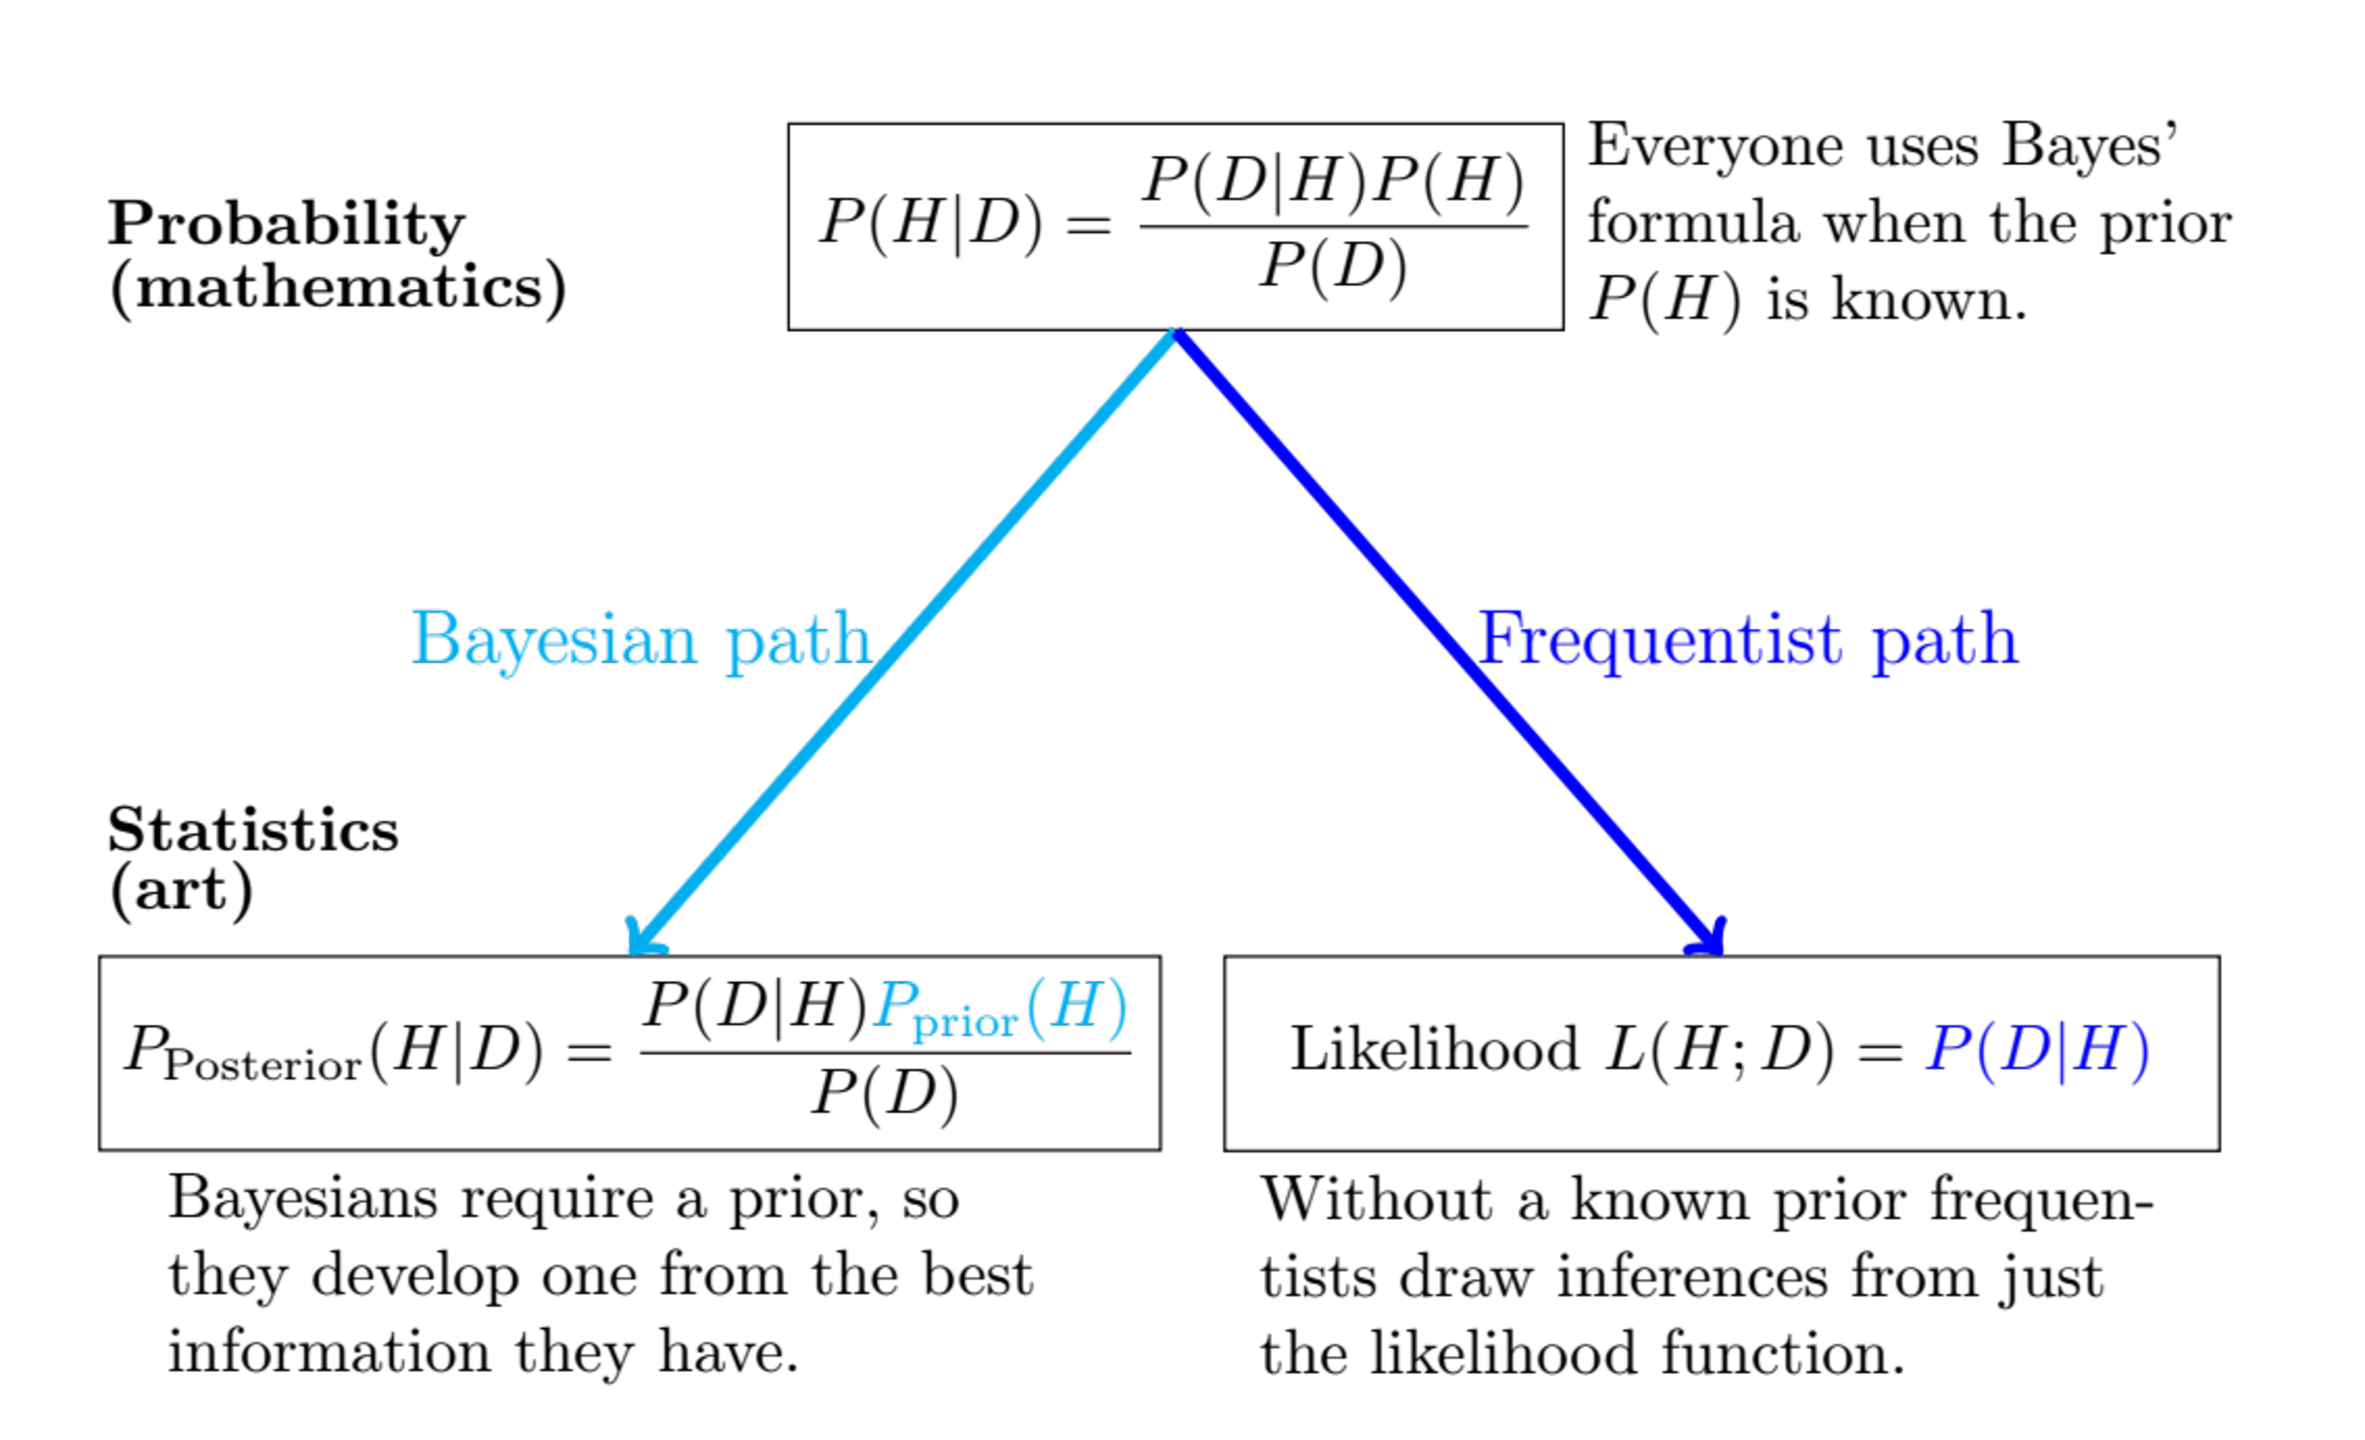
\includegraphics[width=10.5cm]{diagram}\\
	\resizebox{1\hsize}{!}{\underline{source:} Philippe Rigollet. 18.650 Statistics for Applications. Fall 2016. Massachusetts Institute of Technology: MIT OpenCourseWare, \url{https://ocw.mit.edu}. License: Creative Commons BY-NC-SA.}
\end{frame}

\section{Random Variables and univariate distributions}
  {
     \begin{frame}
     \frametitle{Contents}
     \tableofcontents[currentsection]
     \end{frame}
  }
\begin{frame}{Random variables (formal definition)}
    \begin{itemize}
        \item You are probably already at least vaguely aware that random variables are functions, but usually ignore this fact in practice.
        \item Let's take another look at the definition of random variables, given the theoretical background we have just established.
    \end{itemize}
    \begin{definition}[Random Variables]
        Consider a probability space $(\Omega,\mathcal{F},\pr)$ and a measurable space $(\Omega',\mathcal{E})$, i.e. $\Omega'$ is a nonempty set and $\mathcal{E}$ a $\sigma$-algebra over $\Omega'$.\\ A \textbf{random variable} with values in $(\Omega',\mathcal{E})$ is any measurable function $$X:\Omega\longrightarrow\Omega',\quad \omega\mapsto X(\omega)\,,$$
        i.e. any function $X:(\Omega,\mathcal{F})\longrightarrow(\Omega',\mathcal{E})$ with $$\forall E\in\mathcal{E}:\quad X^{-1}(E):=\{\omega\in\Omega\vert X(\omega)\in E\}\in\mathcal{F}\,.$$
    \end{definition}
\end{frame}
\begin{frame}{Visualizing random variables}
       \begin{center}
       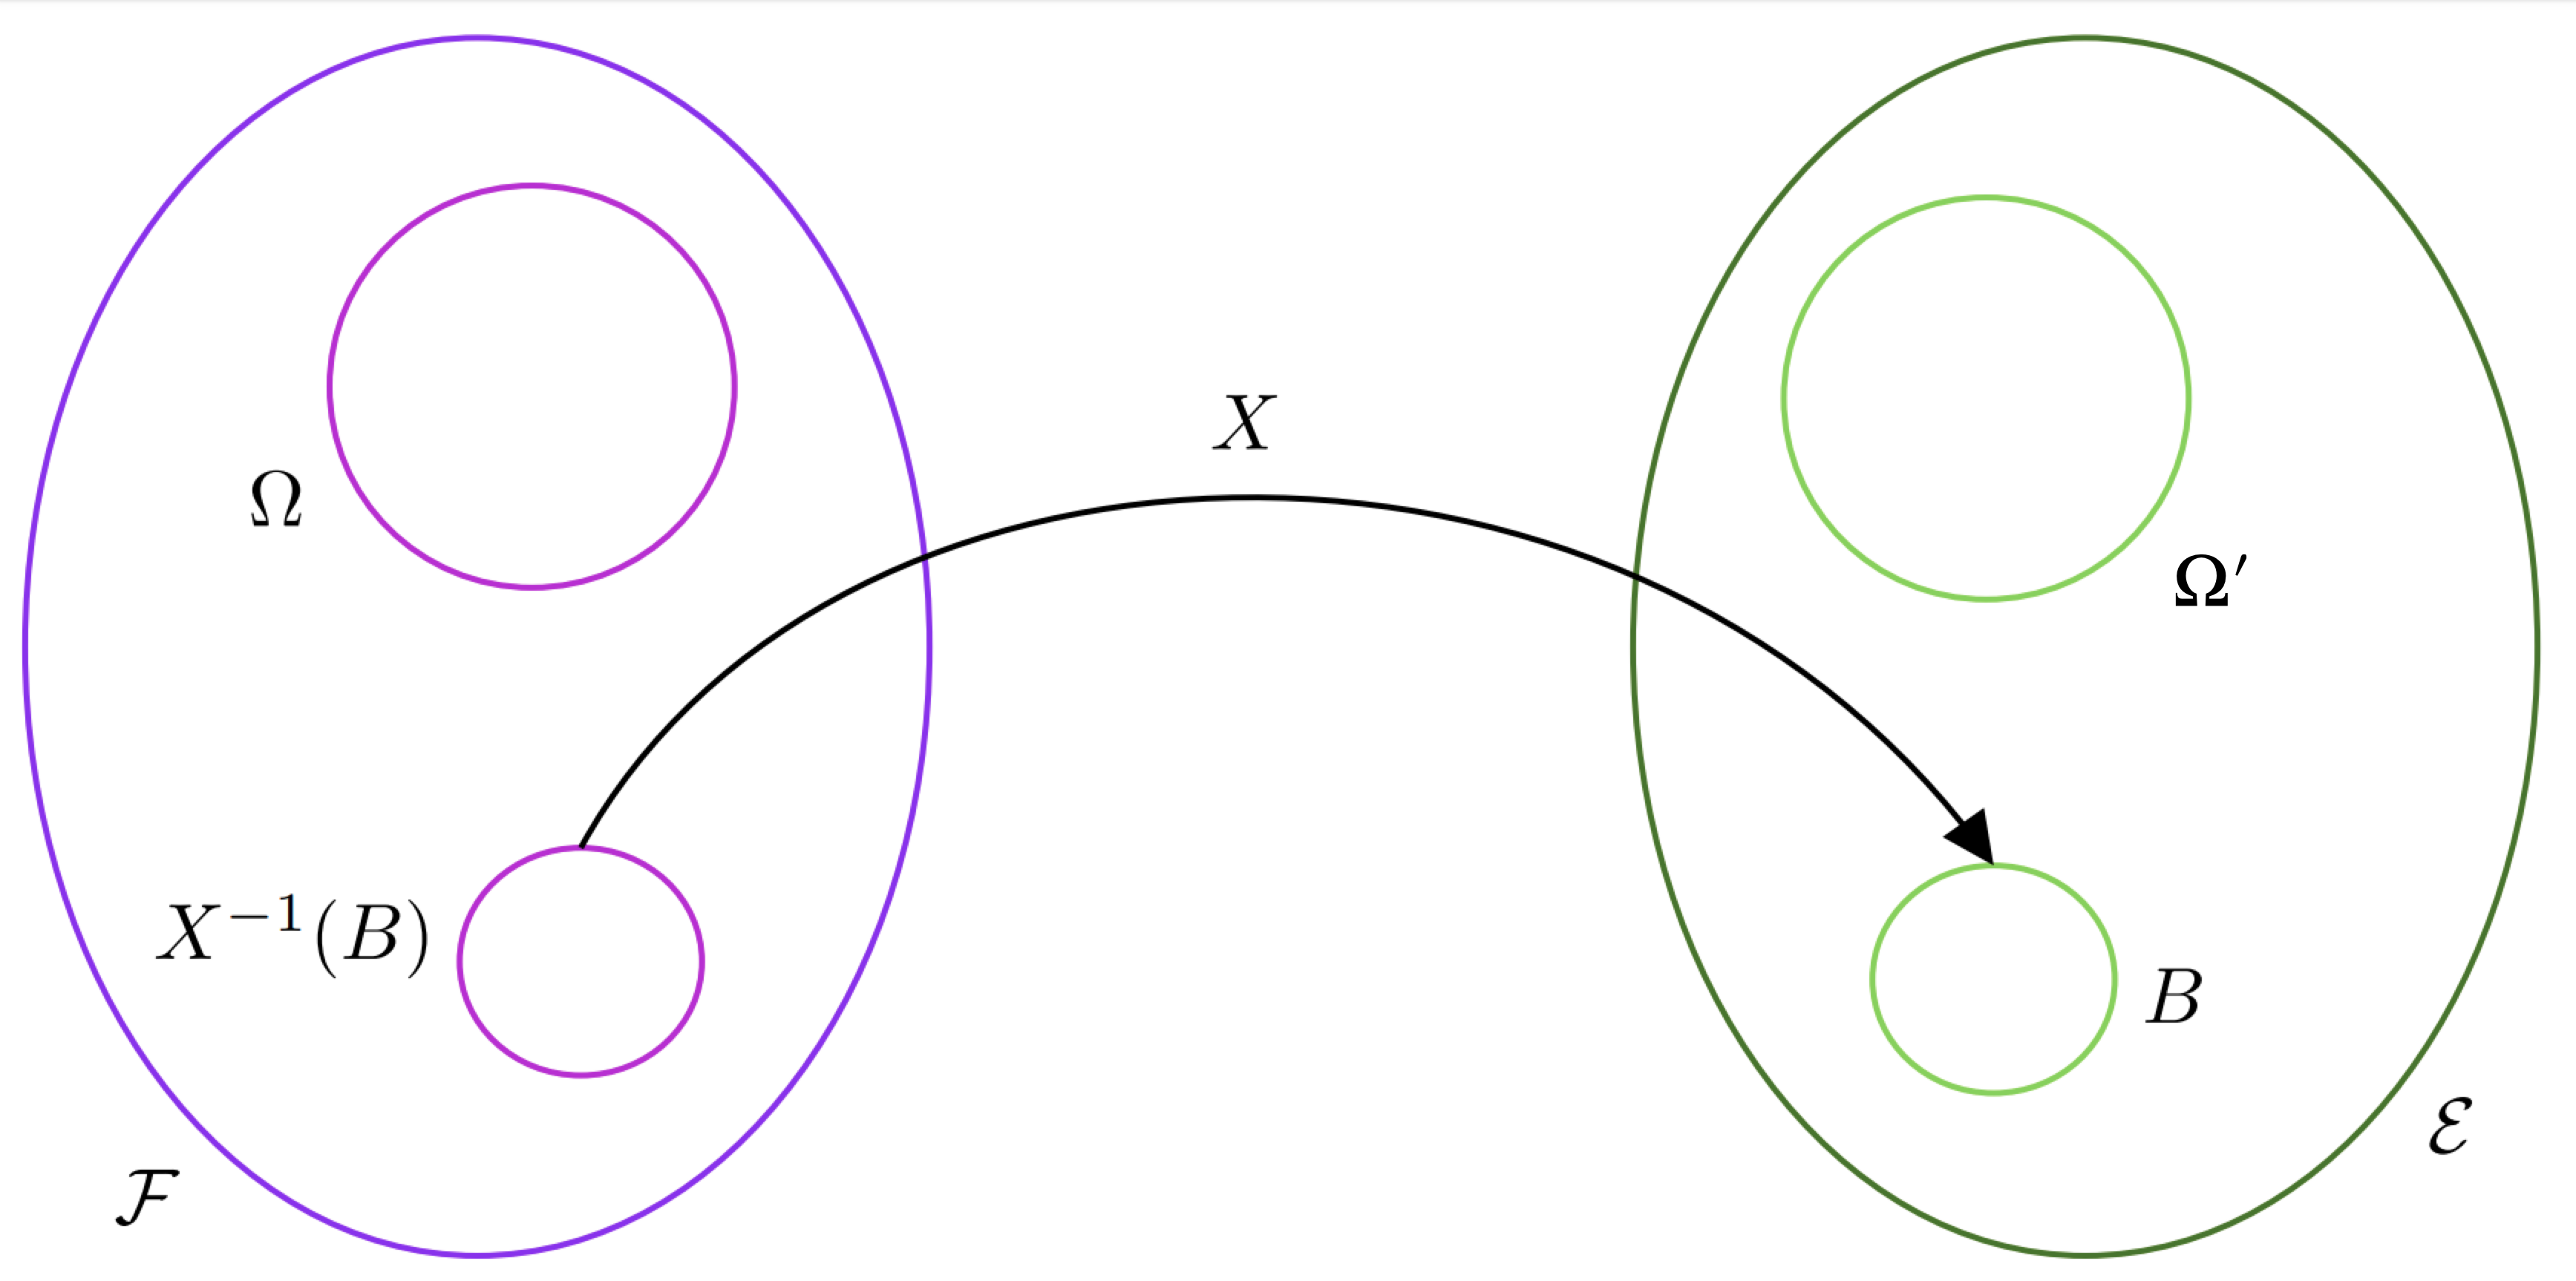
\includegraphics[width=\linewidth]{graphics/RandomVariable1.png}\bigskip\\
       {\tiny \textbf{Source:} \url{https://maurocamaraescudero.netlify.app/post/visualizing-measure-theory-for-markov-chains/}}
   \end{center} 
\end{frame}


\begin{frame}[allowframebreaks]{Usual choices for $(\Omega',\mathcal{E})$}
    \begin{itemize}
        \item Statisticians almost exclusively deal with \textbf{real random variables}, i.e. random variables that take values in $\R$ (or, depending on an authors definition $\R^p,\,p\in\N$) - we too will only consider real random variables from here on out.
        \item While this course's objective is to cover \emph{multivariate statistics}, we will focus on one dimensional random variables in this lecture (i.e. $X:\Omega\longrightarrow\Omega'\subseteq\R$) and extend to higher dimensions a bit later.
        \item Fundamentally, we will usually deal with two different ''kinds'' of random variables:\end{itemize}\pagebreak
        \begin{itemize}
            \item \textbf{Discrete random variables} have a countable image $\Omega'\subseteq\R$, such as the natural numbers $\N$.\footnote{Technically, there is an alternative construction option - ask about it if you are interested ;)}\smallskip \\
            The power set $\mathcal{P}(\Omega')$ is usually chosen as the corresponding $\sigma$-algebra.
            \item \textbf{Continuous random variables} have image $\Omega'=\R$ and\footnote{Having $\Omega'=\R$ is not technically a sufficient condition for a random variable to be continuous, they also need a suitable density - more on that later.} the \emph{Borel $\sigma$-algebra} $\mathcal{B}(\R)$ is usually chosen as the corresponding $\sigma$-algebra.\medskip\\\begin{itemize}
                \item There is some more complex theory behind Borel- sets and $\sigma$-algebras, but for the purposes of this lecture you may simply remember the following:\vspace{-.5cm}\\
                \item  $\mathcal{B}(\R)$ is the $\sigma$-algebra generated by the open sets, i.e., if $\mathcal{O}$ denotes the collection of all open subsets of $\R$, then $\mathcal{B}(\R)=\sigma(\mathcal{O})$.
            \end{itemize}
        \end{itemize}
    
\end{frame}


\begin{frame}{Distributions (formal definition)}
    \begin{itemize}
        \item At first glance, this formal definition might seem a little unnecessarily complicated, but this formal set up gives rise to all kinds of relevant properties and results that are constantly used in applied statistics!
        \item The same goes for the formal definition of distribution:
        \begin{definition}[Distributions]
            Given a probability space $(\Omega,\mathcal{F},\pr)$ and a random variable $X$ with values in $(\Omega',\mathcal{E})$, we define the \textbf{distribution} of $X$ as the probability measure $$\pr_X :=\pr \circ X^{-1}\,,$$
i.e. a function $P_X:\mathcal{E}\longrightarrow [0,1]$.
        \end{definition}
    \end{itemize}
\end{frame}
\begin{frame}{Visualizing formal distributions}
           \begin{center}
       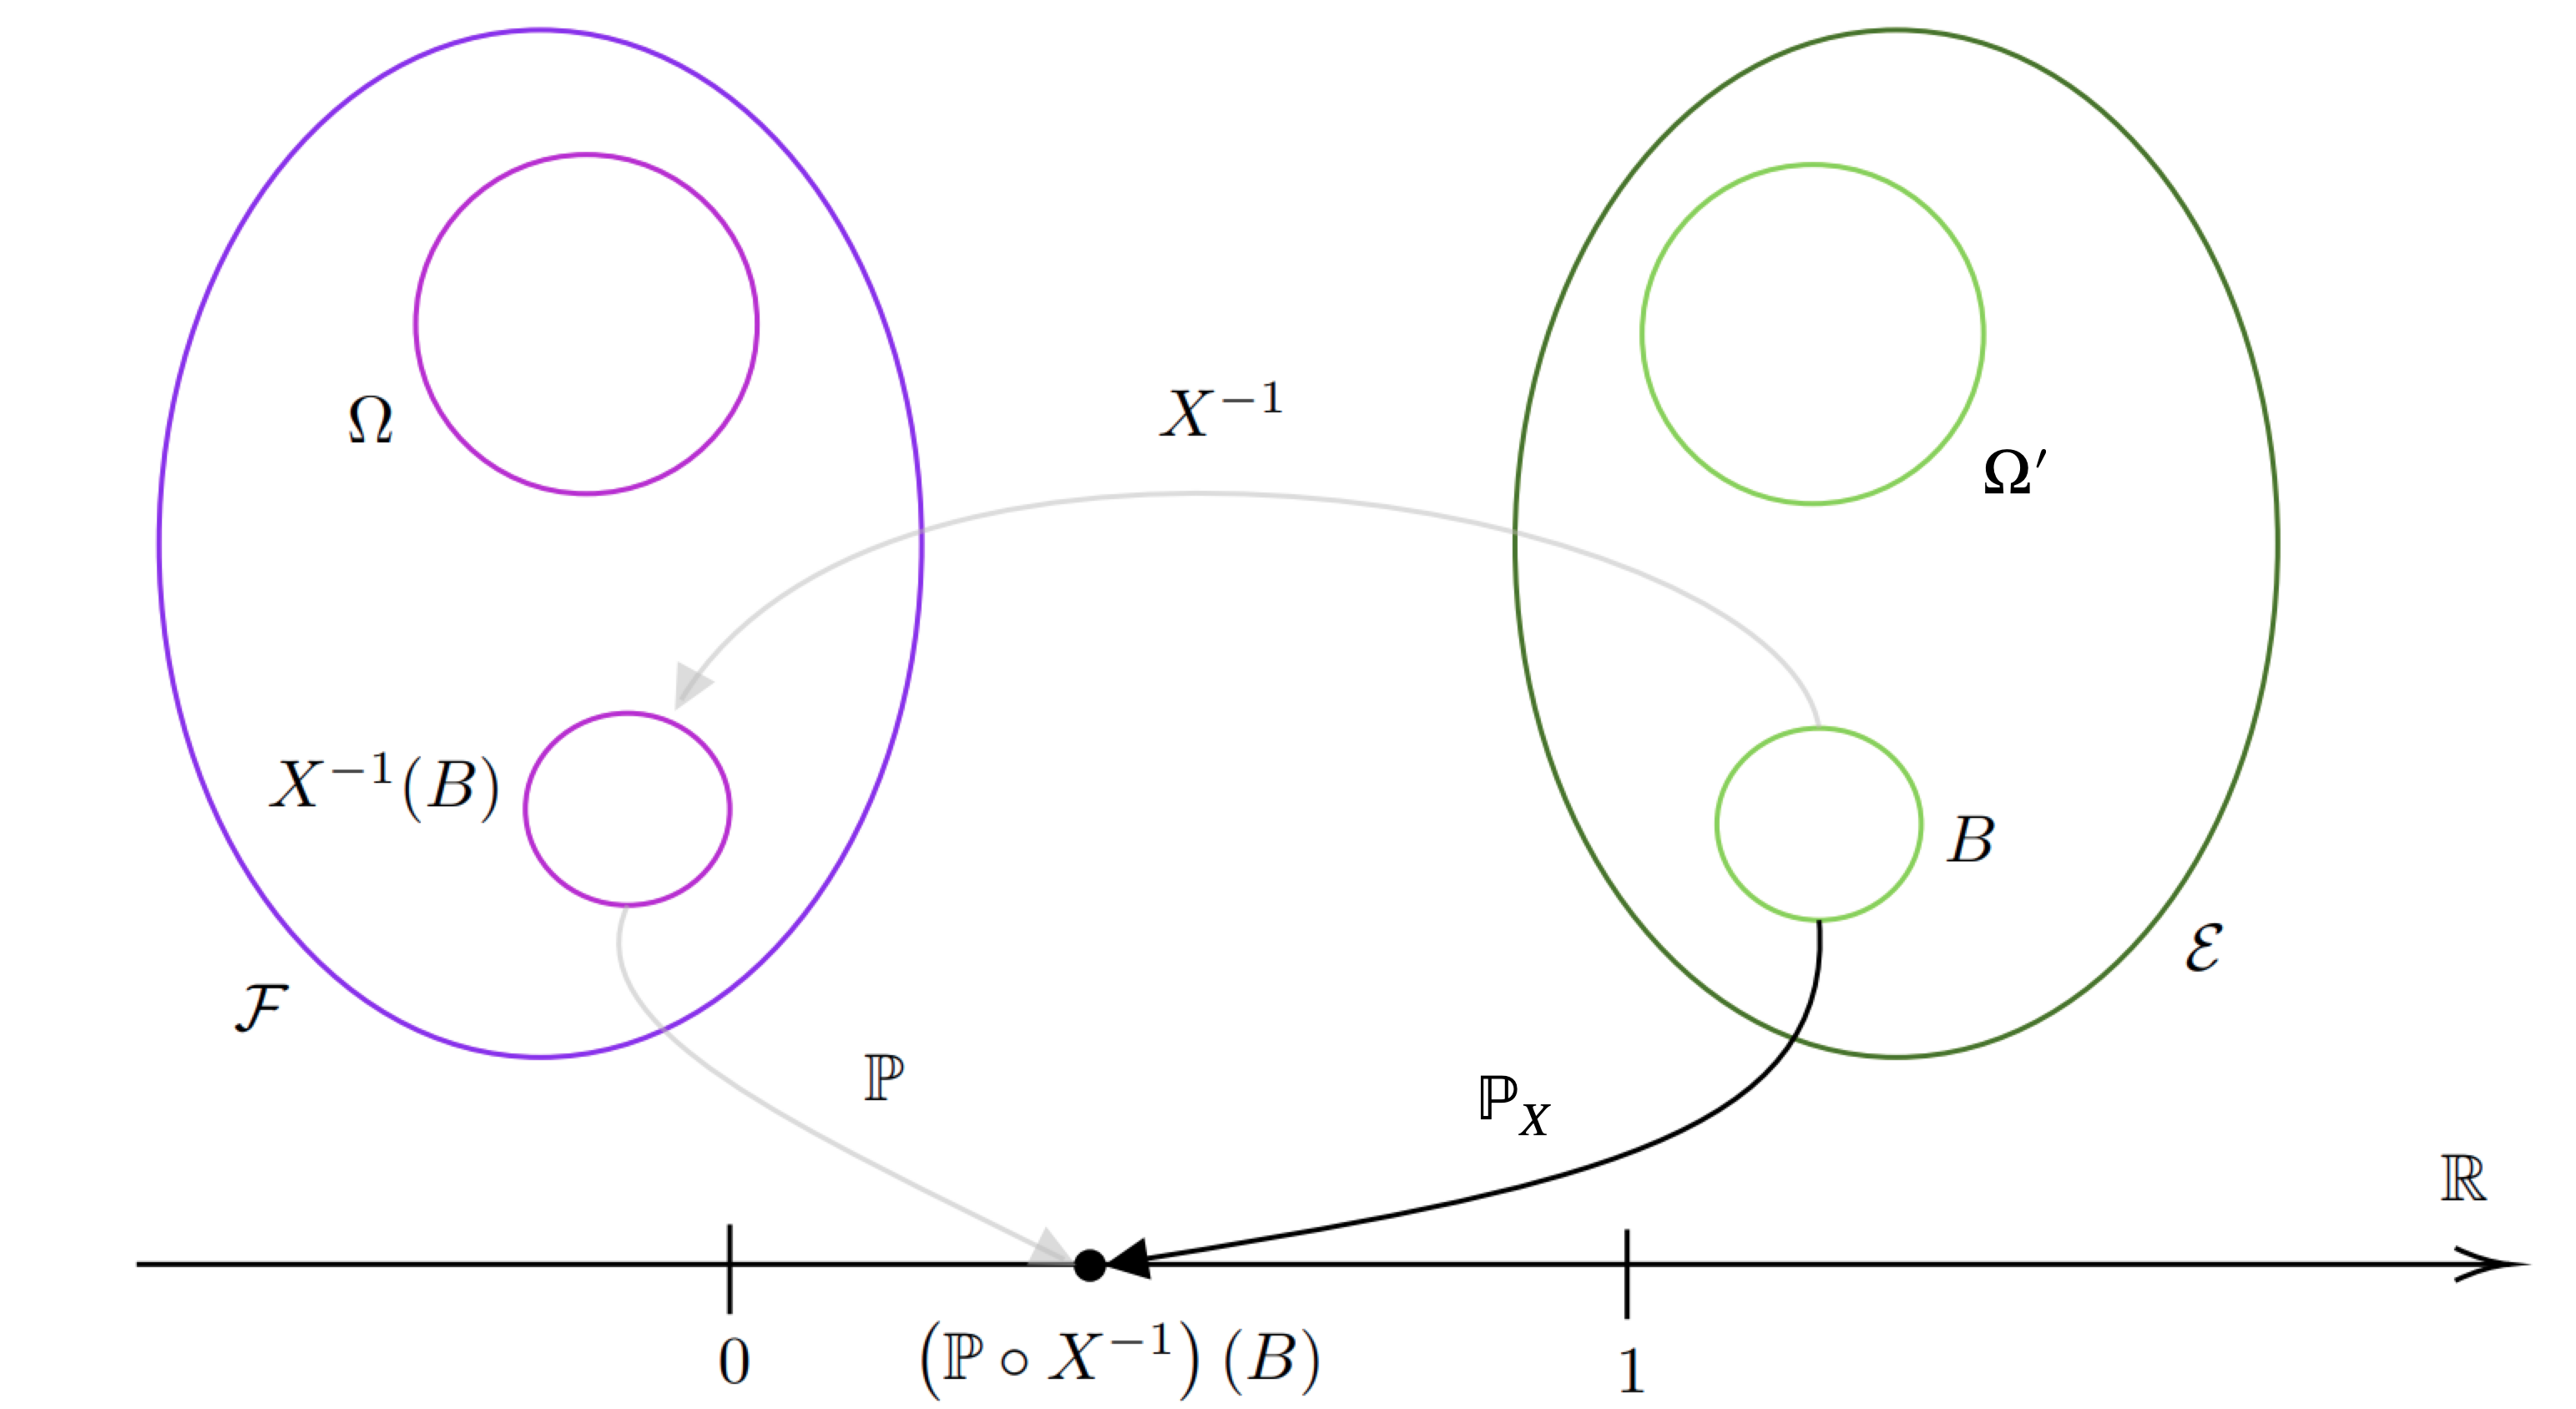
\includegraphics[width=\linewidth]{graphics/ProbabilityDistribution.png}\bigskip\\
       {\tiny \textbf{Source:} \url{https://maurocamaraescudero.netlify.app/post/visualizing-measure-theory-for-markov-chains/}}
   \end{center} 
\end{frame}
\begin{frame}{Distributions as we routinely use them}
    \begin{itemize}
    \item You are probably already familiar with the \textbf{cumulative distribution function (CDF)} $F(x)\equiv \pr(X\leq x)$ of a random variable $X$.
        \item Given the established formal definition of distribution, we can now understand the formal definition of CDF as, for a probability space $(\Omega,\mathcal{F},\pr)$ and random variable $X$ with values in $(\Omega',\mathcal{E})$:
        $$F(x):= \pr_X([-\infty,x])=\pr\big(\{\omega\in\Omega\vert X(\omega)\leq x\}\big)\quad \forall x\in\R\,.$$
    \item The common notation $\pr(X\leq x)$ is therefore a simplification of the term $\pr\big(\{\omega\in\Omega\vert X(\omega)\leq x\}\big)$.
    \end{itemize}
\end{frame}
\begin{frame}[allowframebreaks]{How is $\pr(X\leq x)$ calculated?}
\vspace{-.4cm}
    \begin{itemize}
        \item The general idea for calculating $\pr(X\leq x)$ is to calculate it as in interval $\int_{-\infty}^x\diff\pr_X$, which is defined separately for continuous and discrete random variables:
        \begin{definition}
          For a \textcolor{blueberry}{discrete random variable} $X$, we have neatly chosen a construction where $X$ has the \textbf{countable} image $\Omega'$. \\So, given the function $p:\R\longrightarrow[0,1],\, x\mapsto \pr_X(\{x\})$ with support $\supp(p)\equiv\{x\in\R:$ $p(x)\neq0\}\subset\Omega'$, we have $$
            F(x)=\int_{-\infty}^x\diff\pr_X=\underset{a\in [-\infty,x]\cap\supp(p)}{\sum}p(a)\,.$$
            The function $p$ is referred to as \textbf{probability (mass) function}. \\Note that, by definition, we automatically get $\underset{x\in\supp(p)}{\sum}p(x)=1$.
        \end{definition}

        \begin{definition}
          For a \textcolor{blueberry}{continuous random variable} $X$, we have$$
            F(x)=\int_{-\infty}^x\diff\pr_X=\int_{-\infty}^x f(x)\diff\lambda(x)\,,
            $$ where $\lambda$ denotes the \emph{Lebesgue measure} and $f$ the \textbf{probability density function}, often simply density, defined as the derivative of the CDF.\smallskip\\
            Formally, we say that a probability measure has a density w.r.t. the Lebesgue measure $\lambda$, if the CDF $F$ is absolutely continuous w.r.t. $\lambda$ and then $f(x):=\frac{\partial F(x)}{\partial x}$.
        \end{definition}
{\tiny Note that we now have, by definition of $\pr_X$, that any density $f$ \textbf{must} be a function $f:\R\longrightarrow\R$ with $f(x)\geq 0\,\,\forall x\in\R$ and $\int_\R f(x)\diff x\big(\equiv\int_\R f(x)\diff \lambda (x)\big)\,=1$, which is the commonly taught definition of density.}

    \end{itemize}
\end{frame}


\begin{frame}[fragile]{Example: Normal and Poisson distributions}
 \vspace{-.4cm}   \begin{code}
library(dplyr)
library(tidyr)
library(ggplot2)

x<-seq(0,10,by=0.001)
df<-data.frame(x=rep(x,2),which=c(rep("probability density/
        mass function",length(x)),rep("CDF",length(x))))
df$pois<-c(dpois(x,6),ppois(x,6))
df$norm<-c(dnorm(x,5,2.5),pnorm(x,5,2.5))

df<-gather(df,dist,value,3:4) %>% as.data.frame()

ggplot(df,aes(x,value, colour = dist))+geom_line()+ 
  theme_bw()+scale_x_continuous(breaks=0:10)+
  ylab("")+theme(legend.position="bottom")+
  facet_wrap(~which)
    \end{code}
\end{frame}

\begin{frame}
        \hspace*{-.07\linewidth}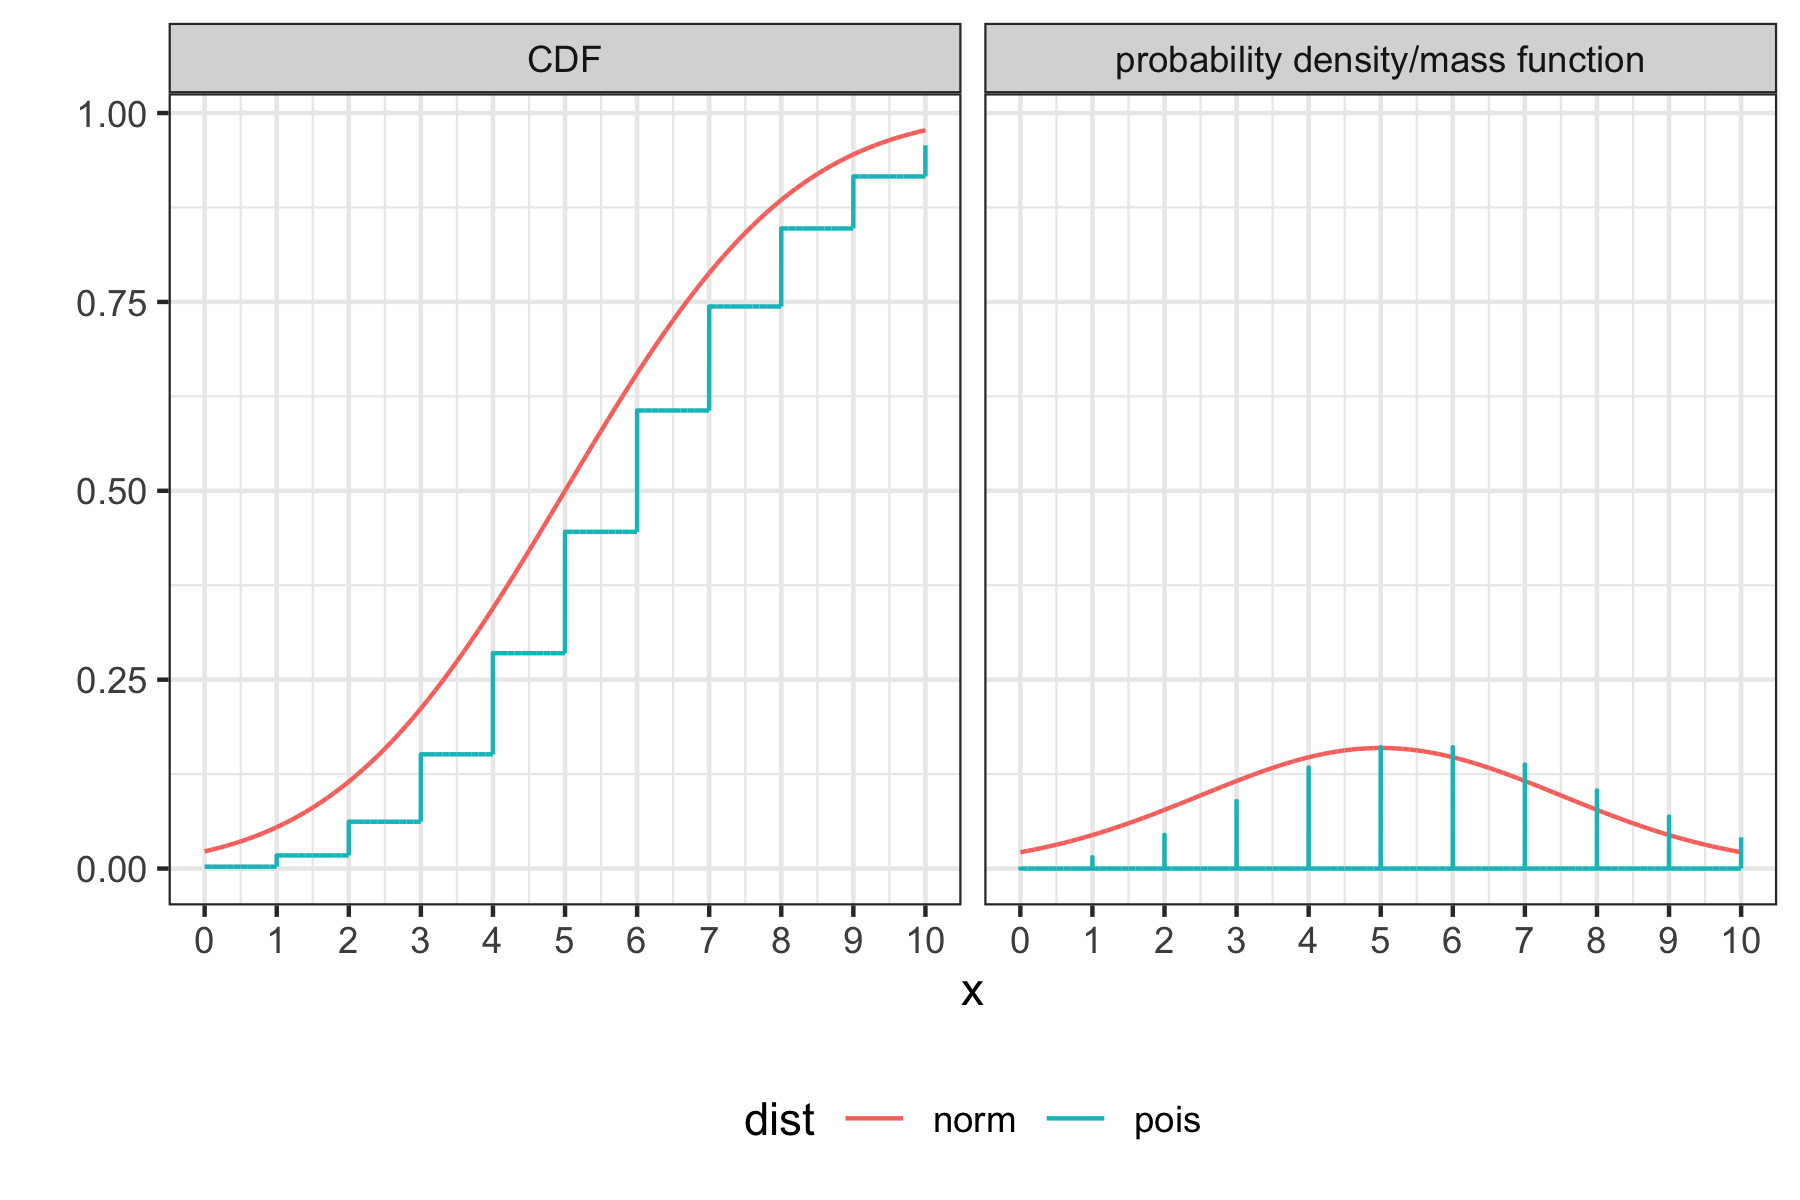
\includegraphics[width=1.1\linewidth]{graphics/cdf.png}
\end{frame}



\begin{frame}[allowframebreaks]{Outlook: Probabilistic modelling for regression}
Let's quickly consider how probabilistic thinking comes into play for the most simple of linear regressions. \emph{\small (This will be discussed in more detail later!)}\bigskip\\
\begin{itemize}
	\item Setting: we would like to model an outcome variable $Y$ as a \textbf{linear} function of some regressor $X$.
	\item Probably you have seen \begin{equation*}
		y_i=\beta_0+\beta_1x_i+\varepsilon_i\,,
	\end{equation*}
where $\varepsilon_i$ is an error term.\\
	\item Now, one approach to solving this problem (i.e. finding values for $\beta_0$ and $\beta_1$) is simply minimizing the error terms with regards to some loss function.
\end{itemize}
	If we choose squared loss, we get the popular OLS, i.e. minimizing the sum of squares in the following graphic:\begin{center}
		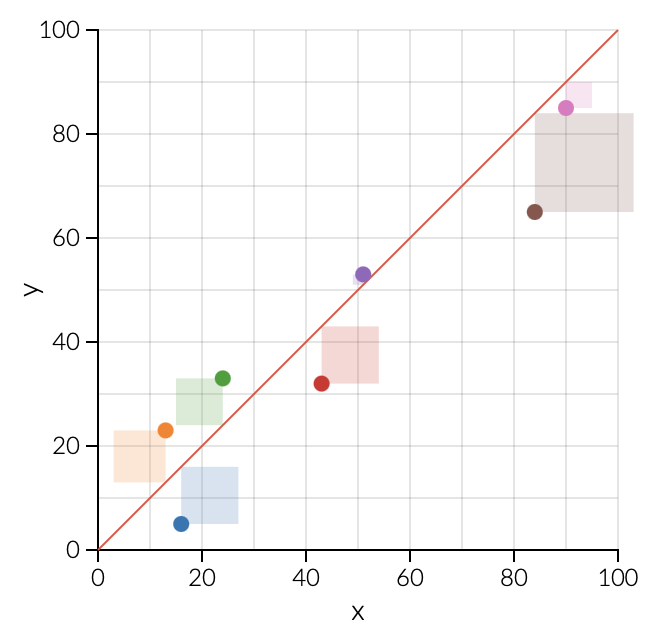
\includegraphics[width=0.4\linewidth]{OLS.png}
	\end{center}
(screenshotted from \href{https://setosa.io/ev/ordinary-least-squares-regression/}{a very cool interactive post on OLS}).

\begin{itemize}
	\item For the OLS solution, which we will talk more about in the next lecture, no probabilistic modelling is required at all!
	\item However, our interpretation is technically also limited - how would we phrase predicitions based on this? \\{\small(\textcolor{blueberry}{keywords: causal inference; probabilistic modelling})}
	\item Now, let's consider the following setting:  \begin{equation*}
		y_i=\beta_0+\beta_1x_i+\varepsilon_i\,,
	\end{equation*} with $\varepsilon_i\overset{i.i.d.}{\sim}N(0,\sigma^2)$.
\item It immediately follows that we consider the $y_i$ to be realizations of a random variable $Y\sim N(\mathbb{E}[Y\vert X],\sigma^2)$ with \begin{equation*}
	\mathbb{E}[Y\vert X]=\beta_0+\beta_1X\,.
\end{equation*}
\item Now, if we take a frequentist view of things - \textcolor{blueberry}{\emph{do not worry, this will be discussed more later}} - all our information is given by the \textcolor{blueberry}{\textbf{Likelihood}}\begin{align*}
	\mathcal{L}\Big(y;\beta=(\beta_0,\beta_1)^\top\Big)&=\prod_{i=1}^n {\frac {1}{\sigma {\sqrt {2\pi }}}}e^{-{\frac {1}{2}}\left({\frac {y_i-(\beta_0+\beta_1x_i) }{\sigma}}\right)^2}\\
	&=\left(\frac{1}{\sigma {\sqrt {2\pi }}}\right)^n e^{\sum_{i=1}^n -{\frac {1}{2}}\left({\frac {y_i-(\beta_0+\beta_1x_i) }{\sigma}}\right)^2}
\end{align*}
and we find suitable estimates for $\beta_0$ and $\beta_1$ by maximizing the Likelihood $\Rightarrow \hat{\beta}=\underset{\beta=(\beta_0\beta_1)^\top\in\R^2}{\operatorname{arg max}}\mathcal{L}(y;\beta)=\underset{\beta=(\beta_0\beta_1)^\top\in\R^2}{\operatorname{arg max}}\log\big(\mathcal{L}(y;\beta)\big)$.

\item This results in (we will look at the general Maximum Likelihood transform for linear regression later) \begin{align*}
\hat{\beta}_1&=\frac{\sum_{i=1}^n\left(x_i-\bar{x}\right)\left(y_i-\bar{y}\right)}{\sum_{i=1}^n\left(x_i-\bar{x}\right)^2}\\
\hat{\beta}_0&=\bar{y}-\hat{\beta}_1\bar{x}\\
\sigma^2&=\frac{1}{n}\sum_{i=1}^n (y_i-(\hat{\beta}_0+\hat{\beta}_1x_i))^2
\end{align*}
\item We will later see that the maximum likelihood estimates $\hat{\beta}_0$ and $\hat{\beta}_1$ are the same as the OLS ones for linear regression!
\end{itemize}\pagebreak
\begin{itemize}
\item But, a cool thing about specifically specifying the model using probabilistic tools is that we can then say \begin{center}
	"\emph{For an observed $X$-value $x_{\text{value}}$, we predict the expectation of the target variable $Y$ to be equal to $\hat{\beta}_0+\hat{\beta}_1x_{\text{value}}$}".
\end{center}
	\item Still, we should never loose sight of all the assumptions that we are making! What are they in our specific example?
\end{itemize}
\end{frame}


\begin{comment}
\section{Combining theory and practice: Another regression-example}
  {
     \begin{frame}
     \frametitle{Contents}
     \tableofcontents[currentsection]
     \end{frame}
  }
\begin{frame}{}
    \begin{itemize}
        \item 
    \end{itemize}
\end{frame}
\end{comment}

\end{document}